\begin{flushleft}
\section{Joint Board Boosterpack}
\end{flushleft}
\label{app:joint_board_boosterpack}
\begin{figure}[H]
	\centering
	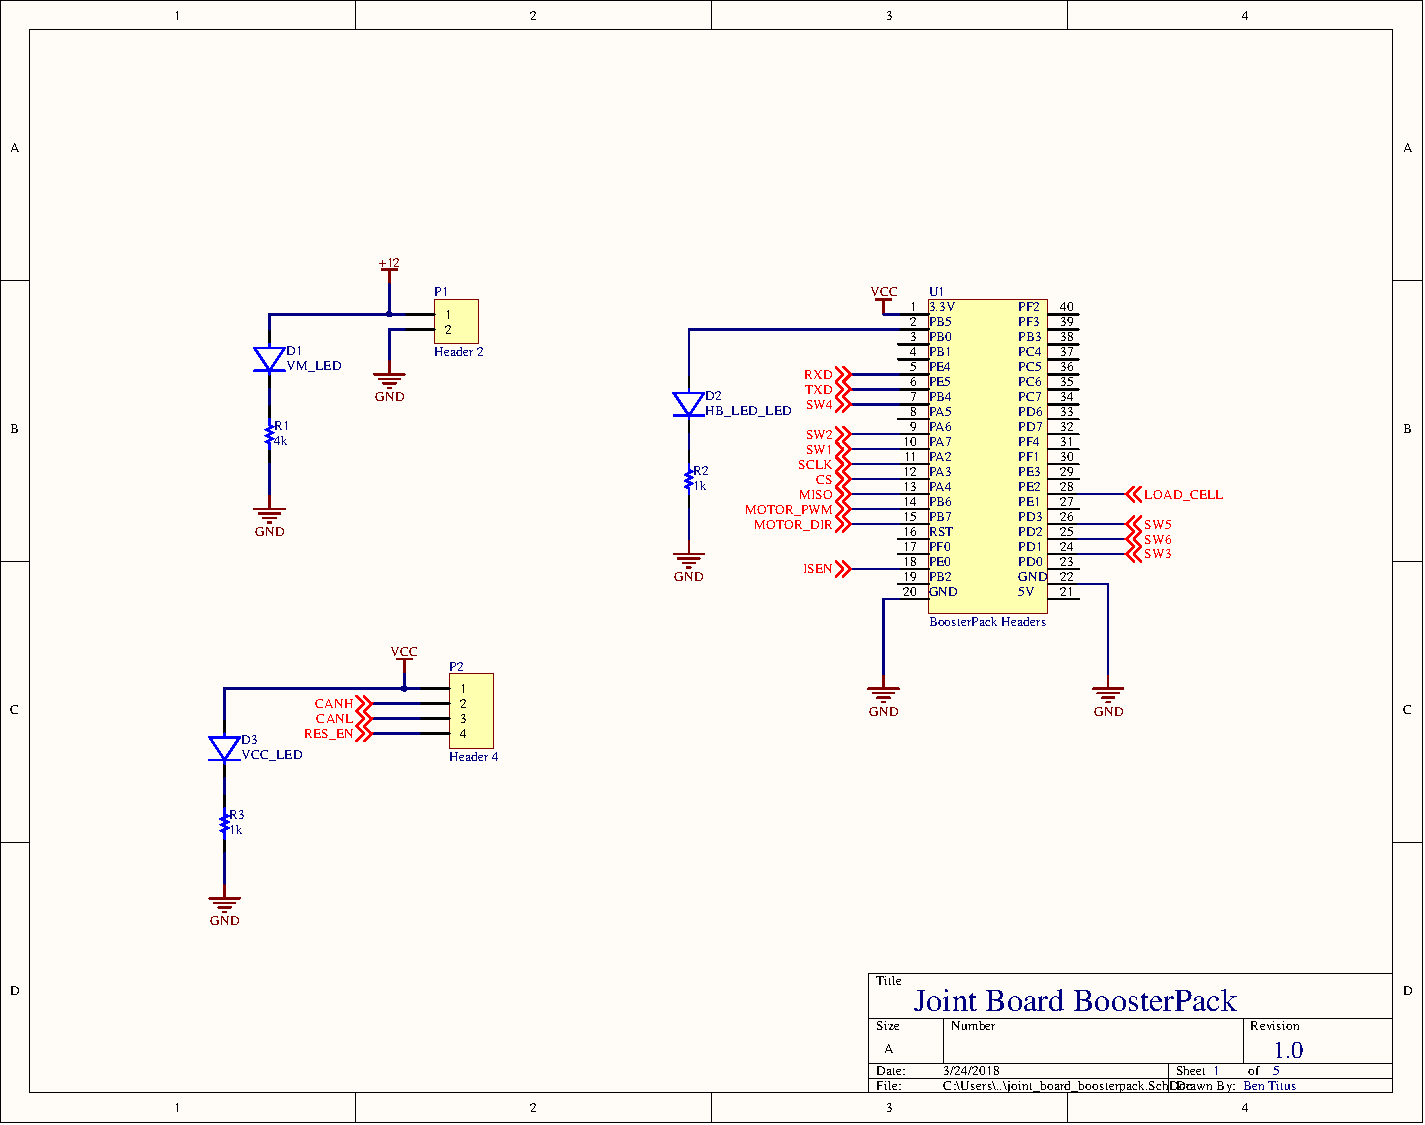
\includegraphics[page=1,scale=0.8,angle=270]{PDFs/joint_board_boosterpack.PDF}
	\caption{Circuit diagram for joint board Boosterpack PCB}
	\label{fig:joint_board_boosterpack_circuit1}
\end{figure}
\begin{figure}[H]
	\centering
	\includegraphics[page=2,scale=0.8,angle=270]{PDFs/joint_board_boosterpack.PDF}
	\caption{Circuit diagram for joint board Boosterpack PCB}
	\label{fig:joint_board_boosterpack_circuit2}
\end{figure}
\begin{figure}[H]
	\centering
	\includegraphics[page=3,scale=0.8,angle=270]{PDFs/joint_board_boosterpack.PDF}
	\caption{Circuit diagram for joint board Boosterpack PCB}
	\label{fig:joint_board_boosterpack_circuit3}
\end{figure}
\begin{figure}[H]
	\centering
	\includegraphics[page=4,scale=0.8,angle=270]{PDFs/joint_board_boosterpack.PDF}
	\caption{Circuit diagram for joint board Boosterpack PCB}
	\label{fig:joint_board_boosterpack_circuit4}
\end{figure}
\begin{figure}[H]
	\centering
	\includegraphics[page=5,scale=0.8,angle=270]{PDFs/joint_board_boosterpack.PDF}
	\caption{Circuit diagram for joint board Boosterpack PCB}
	\label{fig:joint_board_boosterpack_circuit5}
\end{figure}
\begin{figure}[H]
	\centering
	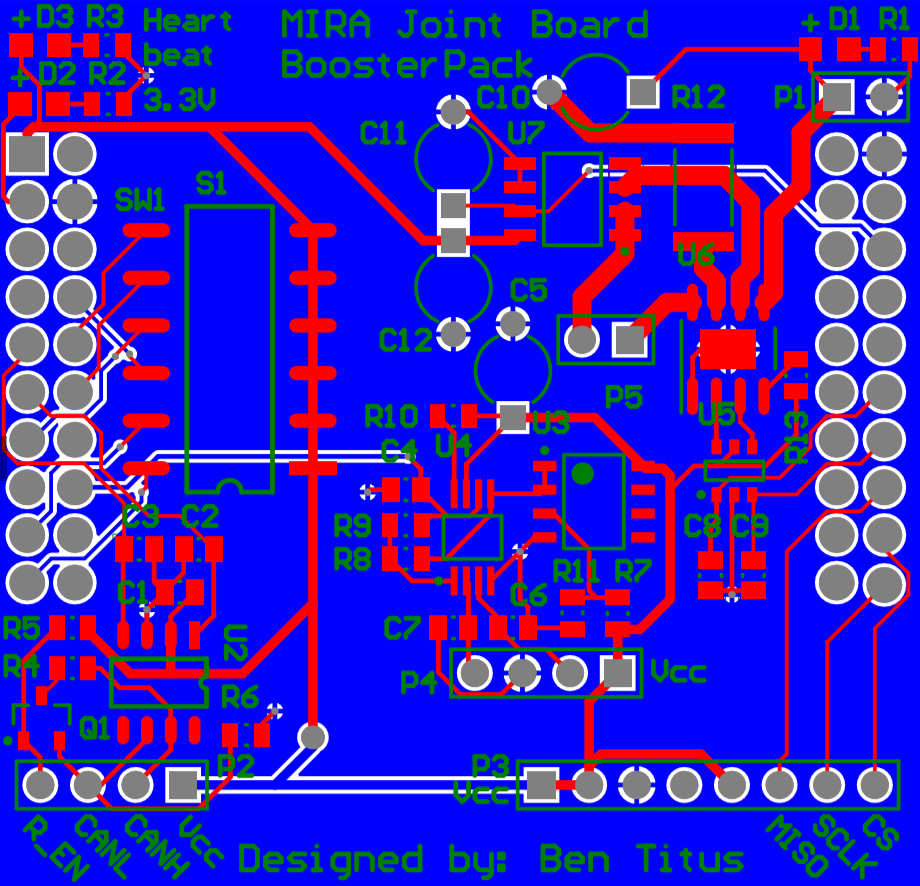
\includegraphics[scale=1]{joint_board_boosterpack} 
	\caption{PCB composite for the joint board Boosterpack PCB}
	\label{fig:joint_board_boosterpack_pcb}
\end{figure}
\begin{figure}[H]
	\centering
	\includegraphics[page=7,width=\textwidth]{PDFs/joint_board_boosterpack.PDF} 
	\caption{Bill of materials for the joint board Boosterpack PCB}
	\label{fig:joint_board_boosterpack_bom}
\end{figure}